\documentclass[stu,letterpaper,12pt,donotrepeattitle,floatsintext]{apa7}
% Preámbulo común de los documentos de Nexus: Normas APA 7.a edición (trabajo de estudiante).
% Se carga con % Preámbulo común de los documentos de Nexus: Normas APA 7.a edición (trabajo de estudiante).
% Se carga con % Preámbulo común de los documentos de Nexus: Normas APA 7.a edición (trabajo de estudiante).
% Se carga con \input{../comun/preambulo} justo después de \documentclass.
\usepackage[spanish,es-noshorthands,es-tabla]{babel}
\usepackage[T1]{fontenc}
\usepackage{newtxtext,newtxmath}
\usepackage{csquotes}
\usepackage[style=apa,backend=biber]{biblatex}
\addbibresource{../comun/referencias.bib}
\usepackage{graphicx}
\usepackage{booktabs}
\usepackage{tabularx}
\usepackage{array}
\usepackage{enumitem}
\usepackage{xurl}
\usepackage{tikz}
\usetikzlibrary{positioning,arrows.meta,shapes.misc}
\hypersetup{hidelinks}
\setlist{itemsep=2pt,topsep=4pt,parsep=0pt}
\setlength{\emergencystretch}{3em}

% Datos de la portada
\authorsnames{Neyder Sebastián Orozco Villamil, Deisy Lorena Jiménez Martínez}
\authorsaffiliations{Universidad Central}
\course{Modelado 3D y Video Juegos (43391312)}
\professor{Mg. Carlos Iván Pinzón Romero}
\duedate{18 de noviembre de 2026}

% Atajos de escritura
\newcommand{\cod}[1]{\texttt{#1}}            % archivos, scripts y código
\newcommand{\ruta}[1]{\textit{#1}}           % rutas de menú: Archivo > Guardar
\newcommand{\tecla}[1]{\textsc{#1}}          % teclas

% Columnas de tabla con texto justificado a la izquierda
\newcolumntype{L}{>{\raggedright\arraybackslash}X}
\newcolumntype{P}[1]{>{\raggedright\arraybackslash}p{#1}}

% Ubicación de figuras y tablas: cerca del texto (los manuales usan H: exactamente en su lugar)
\usepackage{float}
\floatplacement{figure}{!htbp}
\floatplacement{table}{!htbp}
% Nota de figuras y tablas en español y alineada a la izquierda (APA)
\AtBeginDocument{\renewcommand{\notelabel}{Nota}}
\newcommand{\NotaFig}[1]{\if\relax\detokenize{#1}\relax\else\par\raggedright\figurenote{#1}\fi}

% Figura APA: número y título arriba, imagen y nota opcional abajo
%   \Figura[ancho]{archivo}{etiqueta}{título}{nota}
\newcommand{\Figura}[5][0.82\linewidth]{%
  \begin{figure}
    \caption{#4}\label{#3}
    \centering\includegraphics[width=#1]{#2}
    \NotaFig{#5}
  \end{figure}}

% Dos imágenes lado a lado en una misma figura
%   \FiguraDoble{archivo a}{archivo b}{etiqueta}{título}{nota}
\newcommand{\FiguraDoble}[5]{%
  \begin{figure}
    \caption{#4}\label{#3}
    \centering
    \includegraphics[width=0.49\linewidth]{#1}\hfill\includegraphics[width=0.49\linewidth]{#2}
    \NotaFig{#5}
  \end{figure}}

% Tabla APA: número y título arriba; contenido a espacio sencillo y en letra un poco menor
\newenvironment{TablaAPA}[2]{%
  \begin{table}\caption{#2}\label{#1}\centering\small\linespread{1}\selectfont}
  {\end{table}}

% Términos de las referencias como en el manual de normas APA adjunto (Menéndez Echavarría, 2020)
\DefineBibliographyStrings{spanish}{version = {Versión}, nodate = {s.\,f\adddot}}
 justo después de \documentclass.
\usepackage[spanish,es-noshorthands,es-tabla]{babel}
\usepackage[T1]{fontenc}
\usepackage{newtxtext,newtxmath}
\usepackage{csquotes}
\usepackage[style=apa,backend=biber]{biblatex}
\addbibresource{../comun/referencias.bib}
\usepackage{graphicx}
\usepackage{booktabs}
\usepackage{tabularx}
\usepackage{array}
\usepackage{enumitem}
\usepackage{xurl}
\usepackage{tikz}
\usetikzlibrary{positioning,arrows.meta,shapes.misc}
\hypersetup{hidelinks}
\setlist{itemsep=2pt,topsep=4pt,parsep=0pt}
\setlength{\emergencystretch}{3em}

% Datos de la portada
\authorsnames{Neyder Sebastián Orozco Villamil, Deisy Lorena Jiménez Martínez}
\authorsaffiliations{Universidad Central}
\course{Modelado 3D y Video Juegos (43391312)}
\professor{Mg. Carlos Iván Pinzón Romero}
\duedate{18 de noviembre de 2026}

% Atajos de escritura
\newcommand{\cod}[1]{\texttt{#1}}            % archivos, scripts y código
\newcommand{\ruta}[1]{\textit{#1}}           % rutas de menú: Archivo > Guardar
\newcommand{\tecla}[1]{\textsc{#1}}          % teclas

% Columnas de tabla con texto justificado a la izquierda
\newcolumntype{L}{>{\raggedright\arraybackslash}X}
\newcolumntype{P}[1]{>{\raggedright\arraybackslash}p{#1}}

% Ubicación de figuras y tablas: cerca del texto (los manuales usan H: exactamente en su lugar)
\usepackage{float}
\floatplacement{figure}{!htbp}
\floatplacement{table}{!htbp}
% Nota de figuras y tablas en español y alineada a la izquierda (APA)
\AtBeginDocument{\renewcommand{\notelabel}{Nota}}
\newcommand{\NotaFig}[1]{\if\relax\detokenize{#1}\relax\else\par\raggedright\figurenote{#1}\fi}

% Figura APA: número y título arriba, imagen y nota opcional abajo
%   \Figura[ancho]{archivo}{etiqueta}{título}{nota}
\newcommand{\Figura}[5][0.82\linewidth]{%
  \begin{figure}
    \caption{#4}\label{#3}
    \centering\includegraphics[width=#1]{#2}
    \NotaFig{#5}
  \end{figure}}

% Dos imágenes lado a lado en una misma figura
%   \FiguraDoble{archivo a}{archivo b}{etiqueta}{título}{nota}
\newcommand{\FiguraDoble}[5]{%
  \begin{figure}
    \caption{#4}\label{#3}
    \centering
    \includegraphics[width=0.49\linewidth]{#1}\hfill\includegraphics[width=0.49\linewidth]{#2}
    \NotaFig{#5}
  \end{figure}}

% Tabla APA: número y título arriba; contenido a espacio sencillo y en letra un poco menor
\newenvironment{TablaAPA}[2]{%
  \begin{table}\caption{#2}\label{#1}\centering\small\linespread{1}\selectfont}
  {\end{table}}

% Términos de las referencias como en el manual de normas APA adjunto (Menéndez Echavarría, 2020)
\DefineBibliographyStrings{spanish}{version = {Versión}, nodate = {s.\,f\adddot}}
 justo después de \documentclass.
\usepackage[spanish,es-noshorthands,es-tabla]{babel}
\usepackage[T1]{fontenc}
\usepackage{newtxtext,newtxmath}
\usepackage{csquotes}
\usepackage[style=apa,backend=biber]{biblatex}
\addbibresource{../comun/referencias.bib}
\usepackage{graphicx}
\usepackage{booktabs}
\usepackage{tabularx}
\usepackage{array}
\usepackage{enumitem}
\usepackage{xurl}
\usepackage{tikz}
\usetikzlibrary{positioning,arrows.meta,shapes.misc}
\hypersetup{hidelinks}
\setlist{itemsep=2pt,topsep=4pt,parsep=0pt}
\setlength{\emergencystretch}{3em}

% Datos de la portada
\authorsnames{Neyder Sebastián Orozco Villamil, Deisy Lorena Jiménez Martínez}
\authorsaffiliations{Universidad Central}
\course{Modelado 3D y Video Juegos (43391312)}
\professor{Mg. Carlos Iván Pinzón Romero}
\duedate{18 de noviembre de 2026}

% Atajos de escritura
\newcommand{\cod}[1]{\texttt{#1}}            % archivos, scripts y código
\newcommand{\ruta}[1]{\textit{#1}}           % rutas de menú: Archivo > Guardar
\newcommand{\tecla}[1]{\textsc{#1}}          % teclas

% Columnas de tabla con texto justificado a la izquierda
\newcolumntype{L}{>{\raggedright\arraybackslash}X}
\newcolumntype{P}[1]{>{\raggedright\arraybackslash}p{#1}}

% Ubicación de figuras y tablas: cerca del texto (los manuales usan H: exactamente en su lugar)
\usepackage{float}
\floatplacement{figure}{!htbp}
\floatplacement{table}{!htbp}
% Nota de figuras y tablas en español y alineada a la izquierda (APA)
\AtBeginDocument{\renewcommand{\notelabel}{Nota}}
\newcommand{\NotaFig}[1]{\if\relax\detokenize{#1}\relax\else\par\raggedright\figurenote{#1}\fi}

% Figura APA: número y título arriba, imagen y nota opcional abajo
%   \Figura[ancho]{archivo}{etiqueta}{título}{nota}
\newcommand{\Figura}[5][0.82\linewidth]{%
  \begin{figure}
    \caption{#4}\label{#3}
    \centering\includegraphics[width=#1]{#2}
    \NotaFig{#5}
  \end{figure}}

% Dos imágenes lado a lado en una misma figura
%   \FiguraDoble{archivo a}{archivo b}{etiqueta}{título}{nota}
\newcommand{\FiguraDoble}[5]{%
  \begin{figure}
    \caption{#4}\label{#3}
    \centering
    \includegraphics[width=0.49\linewidth]{#1}\hfill\includegraphics[width=0.49\linewidth]{#2}
    \NotaFig{#5}
  \end{figure}}

% Tabla APA: número y título arriba; contenido a espacio sencillo y en letra un poco menor
\newenvironment{TablaAPA}[2]{%
  \begin{table}\caption{#2}\label{#1}\centering\small\linespread{1}\selectfont}
  {\end{table}}

% Términos de las referencias como en el manual de normas APA adjunto (Menéndez Echavarría, 2020)
\DefineBibliographyStrings{spanish}{version = {Versión}, nodate = {s.\,f\adddot}}

\graphicspath{{figuras/}}
\setcounter{tocdepth}{2}

\title{Nexus: Protocolo de emergencia. Desarrollo de un videojuego de terror y sigilo en Unity 6}

\begin{document}
\maketitle

\renewcommand{\contentsname}{Tabla de contenido}
\tableofcontents
\clearpage

\section*{Resumen}
\addcontentsline{toc}{section}{Resumen}

Este documento presenta el desarrollo de \textit{Nexus: Protocolo de emergencia}, un videojuego de
terror y sigilo en tercera persona hecho en Unity~6 con el Universal Render Pipeline como trabajo
final de la asignatura Modelado 3D y Video Juegos. El jugador controla a un técnico de guardia,
encarnado por los avatares 3D de los dos integrantes del equipo, que debe recuperar tres Discos
Duros Maestros en un centro de datos donde los androides de seguridad se volvieron hostiles, antes
de que el sistema de refrigeración colapse. El trabajo se organizó en ocho fases: preparación del
entorno, modelado de objetos y escenarios, personajes y animación, sistemas de juego, inteligencia
artificial, audio, niveles y menús, y exportación. Los escenarios, objetos, texturas y efectos se
generaron con herramientas de editor programadas en C\#, a partir de mapas de texto y de primitivas
de Unity; los personajes se configuraron con el sistema Humanoid y comparten un único controlador
de animación. El resultado es un juego completo de tres niveles con cámaras fijas al estilo del
survival horror clásico, controles tipo tanque, inventario, guardado, armas, cinemáticas, un puzzle
y un jefe final, compilado para Windows, navegador web (WebGL) y Android.

\textit{Palabras clave:} videojuegos, Unity, modelado 3D, avatar Humanoid, inteligencia artificial,
survival horror
\clearpage

\section{Introducción}

El trabajo final de la asignatura pide desarrollar un videojuego 3D en Unity que reúna las mecánicas
vistas en el curso y que funcione en tres plataformas: Windows, navegador web y Android. Entre los
requisitos están al menos tres niveles con progresión lógica, tres Canvas diferenciados, un selector
de personajes con avatares Humanoid, música de fondo, créditos con la imagen institucional, una
explicación del objetivo, temporizador, sistema de vidas o salud, objetos coleccionables con
contador, enemigos con inteligencia artificial autónoma y cuadros de diálogo narrativos.

Para responder a esos requisitos el equipo creó \textit{Nexus: Protocolo de emergencia}, un juego
de terror y sigilo ambientado en el centro de datos de una empresa de tecnología. El juego toma como
referencia los survival horror clásicos \parencite{capcom1996,capcom1999,square1998}: cámaras fijas
que encuadran cada sala, controles tipo tanque, recursos escasos, un inventario con objetos y notas,
y una atmósfera de tensión constante.

Este documento describe el desarrollo del juego de principio a fin, siguiendo las fases de trabajo
definidas al inicio del proyecto. Cada sección explica qué se construyó, cómo se construyó y con qué
herramientas, y se acompaña de capturas del proyecto. El código fuente, las herramientas de editor y
la bitácora detallada del proceso están en el repositorio del proyecto \parencite{repositorio2026}.

\section{Objetivos}

\subsection{Objetivo general}

Desarrollar un videojuego 3D completo de terror y sigilo en Unity, con tres niveles jugables y todas
las mecánicas exigidas por la asignatura, y compilarlo para Windows, navegador web y Android.

\subsection{Objetivos específicos}

\begin{itemize}
  \item Configurar un proyecto de Unity~6 con el Universal Render Pipeline y perfiles de compilación
        para las tres plataformas.
  \item Modelar los objetos y escenarios de un centro de datos con primitivas de Unity, texturas y
        sombreadores propios.
  \item Convertir los avatares 3D de los integrantes en personajes jugables con el sistema de Avatar
        Humanoid y animarlos con un único controlador de animación.
  \item Programar los sistemas de juego: cámaras fijas, controles, salud, temporizador, HUD,
        diálogos, inventario, guardado, habilidades, armas y controles táctiles.
  \item Implementar enemigos con inteligencia artificial basada en una máquina de estados, con
        visión, oído, patrulla y persecución, y un jefe final.
  \item Diseñar y construir tres niveles con objetivos encadenados, un puzzle, cinemáticas y una
        transición animada entre niveles.
  \item Integrar música y efectos de sonido mezclados por capas según la situación del juego.
  \item Compilar y probar las versiones para Windows, WebGL y Android.
\end{itemize}

\section{Metodología}

\subsection{Desarrollo por fases}

El proyecto se dividió en ocho fases (Tabla~\ref{tab:fases}). Cada fase produjo una parte jugable
que se probaba en el editor antes de pasar a la siguiente, de modo que el juego estuvo en estado
ejecutable durante todo el desarrollo. Algunas fases avanzaron en paralelo; por ejemplo, las
compilaciones de prueba para las tres plataformas se hicieron desde el primer día para detectar a
tiempo cualquier limitación de exportación.

\begin{TablaAPA}{tab:fases}{Fases del desarrollo}
\begin{tabularx}{\linewidth}{P{1.2cm}P{4.2cm}L}
\toprule
Fase & Nombre & Contenido \\
\midrule
0 & Preparación del entorno & Instalación de Unity y sus módulos, creación y organización del proyecto, ajustes de compilación y control de versiones \\
1 & Modelado de objetos y entorno & Texturas y sombreadores propios, objetos del centro de datos, utilería y decoración automática \\
2 & Personajes y animación & Avatares de los integrantes, sistema Humanoid, animaciones de Mixamo, personajes secundarios y animaciones creadas por código \\
3 & Sistemas de juego & Cámaras fijas, controles, salud, temporizador, HUD, diálogos, inventario, guardado, habilidades, armas y controles táctiles \\
4 & Inteligencia artificial & Androides de seguridad con máquina de estados y jefe final \\
5 & Audio & Música y efectos, mezcla por capas y sonido 3D \\
6 & Niveles y menús & Constructor de niveles, tres niveles, cinemáticas, menú principal y pantallas finales \\
7 & Exportación & Compilación y prueba en Windows, WebGL y Android \\
\bottomrule
\end{tabularx}
\end{TablaAPA}

\subsection{Construcción por código}

Una decisión central del proyecto fue construir casi todo el contenido con herramientas de editor
programadas en C\#. En lugar de colocar objetos a mano, cada parte del juego tiene una herramienta
en el menú \ruta{Nexus} del editor de Unity que genera texturas, materiales, prefabs, niveles,
interfaz, animaciones o sonidos a partir de datos. Así, un cambio de diseño se aplica en un solo
lugar y basta con volver a ejecutar la herramienta para reconstruir todo lo que depende de él. Esta
forma de trabajo permitió hacer niveles grandes en poco tiempo y mantener la coherencia visual entre
todos los elementos.

\subsection{Pruebas y registro de evidencias}

Cada sistema se probó en el modo Play del editor con recorridos y pruebas automáticas escritas en
C\#: por ejemplo, un técnico controlado por código que recorre un nivel completo, pruebas de
cobertura de las cámaras o mediciones de la mezcla de audio. Los resultados, las decisiones y las
capturas de cada paso se registraron en una bitácora de desarrollo, con capturas numeradas en orden
cronológico, que es la base de este documento. Salvo que se indique otra cosa, todas las figuras son
capturas propias del proyecto. El trabajo del equipo se coordinó en un repositorio de Git alojado en
GitHub \parencite{repositorio2026}.

\subsection{Herramientas}

La Tabla~\ref{tab:herramientas} resume las herramientas y recursos externos utilizados.

\begin{TablaAPA}{tab:herramientas}{Herramientas y recursos utilizados}
\begin{tabularx}{\linewidth}{P{4.4cm}L}
\toprule
Herramienta o recurso & Uso en el proyecto \\
\midrule
Unity 6.6 \parencite{unity2026} & Motor del juego, con Universal Render Pipeline, Input System y AI Navigation \\
C\# & Lenguaje de los scripts del juego y de las herramientas de editor \\
Blender \parencite{blender2026} & Revisión y conversión de modelos (GLB a FBX), reducción de texturas y poses \\
Avaturn \parencite{avaturn2026} & Creación de los avatares 3D de los integrantes a partir de fotografías \\
Mixamo \parencite{mixamo2026} & Animaciones humanoides, androide base y personajes secundarios \\
Sketchfab & Modelos de las armas, con licencia CC BY 4.0 \parencite{ccby40} \\
Pixabay & Música y efectos de sonido, con la licencia de contenido de Pixabay \parencite{pixabaylicencia} \\
FFmpeg \parencite{ffmpeg2026} & Recorte, nivelación y conversión de los sonidos \\
Git y GitHub & Control de versiones y trabajo en equipo \\
Claude Code \parencite{claudecode2026} & Asistencia de programación \\
\bottomrule
\end{tabularx}
\end{TablaAPA}

\section{Concepto y diseño del juego}

\subsection{Historia}

Nexus Corp. es una empresa de tecnología cuyo centro de datos quedó fuera de control durante el
turno de la noche. La actualización de seguridad CERBERUS~7.1, instalada el día 14, alteró a los
androides de seguridad SENTINEL, que empezaron a tratar a cualquier humano como una anomalía, y al
mismo tiempo falló el sistema de refrigeración. El técnico de guardia, Neyder o Deisy según la
elección del jugador, entra al complejo por una puerta de servicio que se sella detrás de él. Para
forzar el reinicio manual del sistema debe recuperar los tres Discos Duros Maestros, uno en cada
sector, antes de que la temperatura del núcleo llegue al 100\,\%. Durante el recorrido encuentra
los cuerpos de un equipo técnico y de una unidad táctica que entraron antes, cuyas notas revelan
que la empresa conocía el fallo. El juego termina cuando el técnico, con los tres discos, fuerza el
reinicio y los registros del día 14 se hacen públicos.

\subsection{Mecánicas principales}

\begin{TablaAPA}{tab:mecanicas}{Mecánicas principales del juego}
\begin{tabularx}{\linewidth}{P{4.2cm}L}
\toprule
Mecánica & Descripción \\
\midrule
Cámaras fijas & Cada sala tiene sus ángulos de cámara y el juego cambia al más adecuado cuando el personaje sale del cuadro o se acerca a un objeto importante \\
Controles tipo tanque & El personaje avanza hacia donde mira y gira sobre sí mismo, sin depender del ángulo de la cámara \\
Sigilo & Los androides ven con un cono de visión que se bloquea con los racks y oyen al jugador cuando corre o dispara \\
Temporizador & La refrigeración se agota con el tiempo; los cartuchos de refrigerante y las válvulas suman tiempo \\
Salud & Tres oportunidades de evasión; se recuperan con bebidas energéticas y barritas de proteína \\
Objetivos encadenados & Fusibles, tarjetas de acceso, puertas sin energía, válvulas y discos que obligan a explorar \\
Inventario y notas & Terminal portátil con objetos, archivo de notas y mapa del nivel \\
Guardado & En las terminales de respaldo, gastando una memoria USB \\
Habilidades & Una habilidad distinta para cada personaje jugable \\
Combate & Cuchillo, pistola y escopeta con munición limitada; disparar hace ruido \\
\bottomrule
\end{tabularx}
\end{TablaAPA}

\subsection{Personajes jugables}

Los dos personajes jugables son los avatares 3D de los integrantes del equipo. Para que elegir uno u
otro cambie la forma de jugar, cada uno tiene una habilidad propia que se activa con la tecla
\tecla{Q} y tiene un tiempo de recarga:

\begin{itemize}
  \item \textbf{Neyder Orozco, técnico de redes (Modelo A)}: el \textit{señuelo de red} lanza un
        repetidor que emite una señal falsa durante 8~s; los androides que estén a menos de 14~m van
        a revisarlo. Recarga de 25~s.
  \item \textbf{Deisy Jiménez, analista de sistemas (Modelo B)}: el programa
        \textit{KILLSWITCH.exe} apaga durante 10~s al androide más cercano que tenga a la vista, a
        menos de 7~m. Recarga de 30~s.
\end{itemize}

\subsection{Estructura de los niveles}

El juego tiene tres niveles que aumentan la dificultad con más androides, menos tiempo y menos
recursos (Tabla~\ref{tab:niveles}). La duración prevista de una partida completa es de unos 15 a
20~minutos.

\begin{TablaAPA}{tab:niveles}{Niveles del juego}
\begin{tabularx}{\linewidth}{P{3.6cm}P{2.2cm}L}
\toprule
Nivel & Tiempo inicial & Planteamiento \\
\midrule
1. Cuarto de Mantenimiento & 7:00 & Tutorial: enseña los controles, las cámaras, el inventario y el guardado. Fusible, tarjeta roja, Disco Maestro 1 y huida hasta el ascensor \\
2. Pasillos de Almacenamiento & 8:00 & Laberinto de racks con luces de emergencia: tarjetas roja y azul, Disco Maestro 2, más androides y munición contada \\
3. Núcleo de Datos & 3:00 & Clímax: sala central simétrica, puzzle de válvulas, Disco Maestro 3, jefe final y reinicio del sistema \\
\bottomrule
\end{tabularx}
\end{TablaAPA}

\section{Desarrollo del proyecto}

% =====================================================================
\subsection{Fase 0: preparación del entorno}

\subsubsection{Motor, módulos y plantilla}

El proyecto se creó en Unity 6.6 (versión 6000.6.3f1) con la plantilla \textit{Universal 3D}, que
usa el Universal Render Pipeline (URP). URP es el sistema de renderizado recomendado para proyectos
que se exportan a móviles y navegadores, porque permite iluminación, materiales con emisión y
posprocesado con un costo controlado. Además del soporte para Windows y Web, se instalaron los
módulos de Android: \textit{Android Build Support}, \textit{Android SDK \& NDK Tools} y
\textit{OpenJDK}, necesarios para generar el APK. Al proyecto se añadieron los paquetes de la
Tabla~\ref{tab:paquetes}.

\begin{TablaAPA}{tab:paquetes}{Paquetes de Unity utilizados}
\begin{tabularx}{\linewidth}{P{4.2cm}L}
\toprule
Paquete & Uso en Nexus \\
\midrule
Universal RP 17.6 & Renderizado, luces, materiales con emisión y posprocesado \\
Input System 1.19 & Teclado, ratón, mando y entradas táctiles \\
AI Navigation 2.0 & Mallas de navegación (NavMesh) y agentes para los androides \\
uGUI y TextMeshPro & Interfaz: menú, HUD, inventario y pantallas finales; texto en el espacio 3D \\
Pipeline & Control del editor desde la línea de comandos para automatizar pruebas y compilaciones \\
\bottomrule
\end{tabularx}
\end{TablaAPA}

\subsubsection{Organización del proyecto y escenas}

Todo el contenido propio se agrupó en la carpeta \cod{Assets/Nexus}, con una subcarpeta por tipo
de recurso: escenas, scripts, herramientas de editor, prefabs, materiales, texturas, modelos,
animaciones, audio, interfaz, datos y perfiles de compilación. Se crearon cuatro escenas, que se
cargan en este orden: \cod{00\_Menu} (menú principal), \cod{01\_Mantenimiento},
\cod{02\_Almacenamiento} y \cod{03\_Nucleo} (Figura~\ref{fig:estructura}).

\Figura[0.9\linewidth]{003_estructura-carpetas-y-escenas.jpg}{fig:estructura}{Estructura de carpetas del proyecto y escenas del juego}{}

\subsubsection{Configuración del reproductor y perfiles de compilación}

En \ruta{Project Settings} \textrightarrow{} \ruta{Player} se configuraron el nombre del producto
(\textit{Nexus}) y de la empresa (\textit{Nexus Team}), y los ajustes propios de cada plataforma
(Figura~\ref{fig:player}): en Windows, ventana redimensionable; en Android, el identificador
\cod{com.nexusteam.nexus}, el compilador IL2CPP con arquitectura ARM64, Android~8.0 como versión
mínima y orientación solo horizontal; en Web, compresión con descompresión de respaldo, para que el
juego funcione en cualquier servidor. Android y Web usan el nivel de calidad \textit{Mobile} y
Windows el nivel \textit{PC}.

\Figura[0.85\linewidth]{004_player-settings-android.jpg}{fig:player}{Ajustes del reproductor para Android}{}

Para generar las tres versiones desde el mismo proyecto se crearon tres perfiles de compilación
(\textit{Build Profiles}): \cod{Nexus\_PC\_Windows}, \cod{Nexus\_Web} y \cod{Nexus\_Android}
(Figura~\ref{fig:perfiles}). Cada perfil guarda la configuración de su plataforma, y cambiar de
plataforma consiste en activar el perfil correspondiente.

\Figura[0.85\linewidth]{005_build-profiles-plataformas.jpg}{fig:perfiles}{Ventana de perfiles de compilación con las tres plataformas}{}

% =====================================================================
\subsection{Fase 1: modelado de objetos y del entorno}

\subsubsection{Herramienta de construcción}

Los objetos del juego se modelaron combinando primitivas de Unity (cubos, cilindros y planos) con
texturas y materiales propios. Todo se genera con la herramienta de editor
\cod{ConstructorFase1}, que agrega al menú \ruta{Nexus} \textrightarrow{} \ruta{Fase 1} los pasos
\textit{Generar texturas}, \textit{Crear materiales} y \textit{Construir prefabs}. Cada objeto queda
guardado como prefab, listo para colocarlo en los niveles.

\subsubsection{Texturas procedurales}

Las texturas se generan por código, píxel a píxel, por lo que son originales. Junto con cada
textura de color se genera un mapa de alturas y, a partir de él, un mapa de normales que da relieve
a la luz: los agujeros se ven hundidos y las asas sobresalen (Tabla~\ref{tab:texturas}).

\begin{TablaAPA}{tab:texturas}{Texturas generadas por código}
\begin{tabularx}{\linewidth}{P{3.6cm}P{2.3cm}L}
\toprule
Textura & Tamaño & Contenido \\
\midrule
Frente de rack & 256 × 1024 & Rieles con agujeros de montaje, diez servidores con malla perforada, etiquetas, huecos para LEDs, botones, asas y rejilla de ventilación \\
Piso técnico & 512 × 512 & Baldosas de 60~cm con tornillos; una de cada cuatro perforada para la ventilación \\
Pared & 512 × 512 & Paneles metálicos con juntas, remaches, banda horizontal y zócalo \\
Franjas de peligro & 256 × 256 & Diagonales amarillas y negras para los marcos de las puertas \\
Metal cepillado & 256 × 256 & Vetas horizontales para el cuerpo de los racks \\
Tarjetas de acceso & 256 × 160 & Banda, chip dorado y logotipo, en rojo y en azul \\
\bottomrule
\end{tabularx}
\end{TablaAPA}

\subsubsection{Sombreador de LEDs}

Para los cientos de luces de los racks se escribió un sombreador propio en HLSL para URP. El
parpadeo se calcula en la tarjeta gráfica a partir del tiempo, sin ningún script, lo que mantiene
el juego fluido en Android y WebGL. Cada LED guarda en el color de sus vértices su color (verde,
azul, ámbar o rojo) y un desfase, de modo que todos los LEDs de un rack forman una sola malla y aun
así cada uno parpadea a su ritmo. El color se multiplica por una intensidad alta para que el efecto
\textit{Bloom} del posprocesado los haga brillar. El mismo sombreador, en modo de pulso suave, se
usa en el neón de los discos, en los lectores de las puertas y en las pantallas de las terminales.

\subsubsection{Objetos del centro de datos}

\begin{itemize}
  \item \textbf{Rack de servidores} (0,6 × 2,0 × 1,0~m): cuerpo de metal cepillado, frente y
        trasera con la textura de rejilla y una malla con 80 LEDs colocados exactamente sobre los
        huecos de la textura (Figura~\ref{fig:rack}, izquierda). Los racks se agrupan en filas de diez,
        combinadas en tres mallas por celda, con lo que un laberinto de cientos de racks se dibuja
        con pocas llamadas a la tarjeta gráfica.
  \item \textbf{Disco Duro Maestro}: cubo metálico con un anillo y placas de neón azul y una luz
        propia; gira y flota, y se recoge al tocarlo (Figura~\ref{fig:rack}, derecha).
  \item \textbf{Tarjetas de acceso} roja y azul, que abren las puertas de su color.
  \item \textbf{Puerta de seguridad}: marco con franjas de peligro, dos hojas que se deslizan y un
        lector cuya luz indica qué tarjeta se necesita (Figura~\ref{fig:puerta}, izquierda). Hay variantes
        roja, azul, libre y sin energía.
  \item \textbf{Terminal}: consola con teclado y monitor con texto real en la pantalla, escrito con
        TextMeshPro en el espacio 3D (Figura~\ref{fig:puerta}, derecha).
  \item \textbf{Módulos de 3 × 3~m} de piso y pared, con los que se arman todos los niveles.
  \item \textbf{Objetos del nivel}: fusible, memoria USB, bebida energética, barrita de proteína,
        cartucho de refrigerante, mesa con nota, panel de fusibles, terminal de respaldo, válvula de
        refrigeración y ascensor. Los objetos que se recogen tienen una leve emisión para distinguirse
        en la oscuridad sin gastar una luz cada uno.
\end{itemize}

\FiguraDoble{014_rack-servidor-detalle.jpg}{015_disco-duro-maestro.jpg}{fig:rack}{Racks de servidores con sus LEDs (izquierda) y Disco Duro Maestro sobre su pedestal (derecha)}{}

\FiguraDoble{016_puerta-seguridad-roja.jpg}{017_terminal-nexus.jpg}{fig:puerta}{Puerta de seguridad roja (izquierda) y terminal con texto en pantalla (derecha)}{}

Los productos de curación tienen un diseño propio, sin marcas reales: una lata de bebida energética
y una barrita de proteína con envoltura de grafito, bordes plateados y una franja turquesa
(Figura~\ref{fig:curacion}).

\Figura[0.6\linewidth]{111_bebida-energetica-y-barrita.jpg}{fig:curacion}{Bebida energética y barrita de proteína}{}

\subsubsection{Utilería y decoración automática}

Para que los escenarios se vean como una empresa abandonada a la fuerza se modelaron 48 objetos de
utilería, también con primitivas y texturas generadas por código (Figura~\ref{fig:utileria}):
escritorios con computadores, sillas, archivadores, casilleros, una consola de cámaras de seguridad,
pizarras y carteles de la empresa; máquinas expendedoras, mesas y una nevera para la cafetería;
estanterías, cajas, bobinas de cable y gabinetes eléctricos para el almacén; y papeles, latas,
bolsas de basura, paneles del techo caídos, manchas, charcos y conos de precaución. Se agregaron
efectos de polvo flotante, chispas y fluorescentes que titilan. Las piezas de cada objeto se
combinan en una sola malla por material para que su costo de dibujo sea bajo.

\FiguraDoble{056_utileria-vitrina-general.jpg}{057_utileria-maquinas-y-escritorios.jpg}{fig:utileria}{Utilería del centro de datos: vitrina general (izquierda) y máquinas expendedoras con escritorios (derecha)}{}

Un decorador automático amuebla cada sala según su tema (oficina, seguridad, cafetería, almacén,
servidores, eléctrico, mantenimiento o pasillo). Primero coloca los muebles obligatorios del tema,
luego llena las paredes que ve la cámara de la sala hasta una densidad definida, cuelga carteles y
gabinetes y, por último, riega basura por el suelo y añade polvo del tamaño de la sala. Los muebles
van siempre contra las paredes, para no estorbar el paso del jugador ni las rutas de los androides,
y nunca junto a una cámara o una puerta. Los muebles altos bloquean la visión de los androides, así
que también sirven para esconderse. La decoración usa una semilla fija: reconstruir un nivel da
siempre el mismo resultado.

Las máquinas expendedoras dan bebidas energéticas y barritas de proteína hasta agotarse, pero el
producto cae con un golpe que atrae a los androides que estén a menos de 11~m, lo que convierte la
curación en una decisión con riesgo.

% =====================================================================
\subsection{Fase 2: personajes y animación}

\subsubsection{Avatares de los integrantes}

Los dos personajes jugables son los avatares de los integrantes del equipo, creados con Avaturn a
partir de fotografías \parencite{avaturn2026}. Se descargaron en formato GLB, que guarda en un solo
archivo la malla, un esqueleto de 52 huesos con nombres estándar y las texturas. Con un script de
Python para Blender \parencite{blender2026} se convirtieron a FBX con las texturas incrustadas, sin
huesos adicionales y con la escala en metros, que es el formato con el que Unity configura los
avatares humanoides.

\subsubsection{Configuración como Avatar Humanoid}

En Unity, los modelos se importaron con el tipo de animación \textit{Humanoid} y la definición
\textit{Create From This Model} (Figura~\ref{fig:rig}). Unity generó un avatar válido para cada
integrante, con los 52 huesos asignados al esqueleto humano estándar (Figura~\ref{fig:avatares}).
El sistema Humanoid traduce el esqueleto de cada modelo a un esqueleto común; gracias a eso, una
misma animación funciona en los dos personajes y en los androides aunque tengan proporciones
distintas, y es lo que permite que el selector de personajes use un único controlador de animación
\parencite{unitymanual2026}.

\Figura[0.75\linewidth]{007_rig-humanoid-neyder.jpg}{fig:rig}{Pestaña Rig del modelo de Neyder con el tipo de animación Humanoid}{}

\FiguraDoble{008_configure-avatar-mapeo-huesos-neyder.jpg}{009_configure-avatar-mapeo-huesos-deisy.jpg}{fig:avatares}{Mapeo de huesos del Avatar Humanoid de Neyder (izquierda) y de Deisy (derecha)}{}

Las texturas se asignaron a materiales URP con mapa de color y de normales. El cabello usa recorte
por transparencia (\textit{alpha clipping}) y se dibuja por las dos caras, una solución más ligera
que la transparencia real para móviles y navegadores; la piel y la ropa usan un flujo de trabajo no
metálico (Figura~\ref{fig:integrantes}).

\Figura[0.85\linewidth]{006_avatares-integrantes-en-unity.jpg}{fig:integrantes}{Avatares de los integrantes en Unity}{}

\subsubsection{Animaciones y controlador}

Los integrantes descargaron de Mixamo \parencite{mixamo2026} las animaciones aplicadas sobre sus
avatares. Se eligieron once clips: reposo, caminar, correr, caminar herido, reacción a un golpe,
golpe al caminar, morir, y reposo, caminar, disparar y apuñalar con arma. Cada clip se configuró
como Humanoid; el avance de la cadera se deja fuera del personaje (\textit{root motion}
descartado), de modo que la animación se reproduce en su sitio y es el componente
\textit{CharacterController} el que mueve al técnico.

El controlador de animación \cod{AC\_Tecnico}, compartido por los dos personajes, tiene un árbol de
mezcla de locomoción (reposo, caminar a 1,8~m/s y correr a 5~m/s) cuyos umbrales coinciden con la
velocidad real de las animaciones, para que los pies no se deslicen sobre el suelo; una variante
herida; los estados de golpe y muerte; y los estados y parámetros de las armas. Al retroceder, la
animación de caminar se reproduce en reversa (Figura~\ref{fig:locomocion}).

\FiguraDoble{022_jugador-animacion-reposo-modo-play.jpg}{023_jugador-caminando-hacia-camara-fija.jpg}{fig:locomocion}{Animación de reposo (izquierda) y el técnico caminando hacia la cámara fija (derecha)}{}

\subsubsection{Personajes secundarios y cadáveres}

De Mixamo se obtuvieron también dos operadores tácticos y un empleado con casco y chaleco, que en
el juego aparecen como los cuerpos de quienes entraron antes que el técnico. Un script de Blender
reduce sus texturas a un máximo de 1024~píxeles, separa los canales de color, normales, rugosidad y
emisión, y combina la rugosidad en el formato que usa el material URP; con esto los archivos pasaron
de hasta 115~MB a unos 10~MB. En Unity se configuraron como Humanoid.

Las poses de los cadáveres se describen con los músculos del sistema Humanoid, valores de $-1$ a 1
que funcionan con cualquier modelo: una pose tendida, tomada del último cuadro de la animación de
muerte, y una pose sentada contra la pared, creada músculo por músculo (piernas al frente, una
rodilla doblada, torso caído y cabeza ladeada). La pose se escribe en los huesos, de modo que el
prefab no necesita un controlador de animación. Cada cuerpo tiene un charco de sangre, una
colisión baja que los androides rodean y una luz tenue para distinguirse en la oscuridad
(Figura~\ref{fig:cadaveres}).

\FiguraDoble{082_cadaveres-tendidos.jpg}{083_cadaveres-sentados-pared.jpg}{fig:cadaveres}{Poses de cadáver tendidas (izquierda) y sentadas contra la pared (derecha), creadas con los músculos del avatar}{}

\subsubsection{Animaciones de la escopeta creadas por código}

Para la escopeta de corredera se crearon animaciones propias a partir de la técnica de manejo real
de este tipo de arma: culata en el hombro, mano fuerte en la empuñadura y mano de apoyo en el
guardamanos; posición de listo con el cañón hacia abajo; retroceso hacia el hombro; bombeo para
cargar el siguiente cartucho; y recarga a la altura de la cadera, empujando los cartuchos uno por
uno.

\begin{enumerate}
  \item Se escribieron por código, músculo por músculo, tres clips Humanoid: listo, apuntar y
        recargar.
  \item Se agregó al controlador una capa \textit{Escopeta} con una máscara de brazos, manos y
        cabeza: las piernas siguen caminando y corriendo con la capa base.
  \item La cinemática inversa (IK) coloca el arma respecto al hombro según la pose y lleva las
        manos a la empuñadura y al guardamanos. El retroceso, el bombeo y el ciclo de cada cartucho
        se calculan con curvas en el código.
  \item La recarga cuesta tiempo real: 0,5~s por cartucho.
\end{enumerate}

\FiguraDoble{088_escopeta-listo.jpg}{089_escopeta-apuntar-derecha.jpg}{fig:escopeta}{Escopeta en posición de listo (izquierda) y apuntando con la mano de apoyo en el guardamanos (derecha)}{}

\Figura[0.7\linewidth]{091_escopeta-recarga.jpg}{fig:escopeta-recarga}{Recarga de la escopeta, cartucho por cartucho}{}

% =====================================================================
\subsection{Fase 3: sistemas de juego}

\subsubsection{Arquitectura}

Los sistemas del juego están repartidos en scripts con una responsabilidad cada uno
(Tabla~\ref{tab:arquitectura}). Los objetos no se conocen entre sí: se comunican mediante métodos
estáticos del HUD (por ejemplo, mostrar un aviso, cambiar el objetivo o abrir un diálogo) y mediante
eventos, como el que anuncia que se recogió un objeto. Así, una terminal no necesita saber cómo se
dibuja un diálogo.

\begin{TablaAPA}{tab:arquitectura}{Scripts principales del juego}
\begin{tabularx}{\linewidth}{P{4.4cm}L}
\toprule
Script & Responsabilidad \\
\midrule
\cod{EstadoPartida} & Datos que pasan de un nivel a otro: personaje elegido, salud, discos, inventario, munición, notas leídas y cuerpos registrados; guardado y carga \\
\cod{NivelNexus} & Temporizador, temperatura, objetivo inicial, Game Over, paso al nivel siguiente y Victoria; calcula la malla de navegación al cargar el nivel \\
\cod{ControladorJugador} & Movimiento con controles tipo tanque mediante un \textit{CharacterController} \\
\cod{VidaJugador} & Las tres oportunidades de evasión, el estado herido y la muerte \\
\cod{InteraccionJugador} e \cod{Interactuable} & Detecta lo que está cerca, muestra la acción disponible y la ejecuta con la tecla de interactuar \\
\cod{GestorCamaras} y \cod{CamaraFija} & Las cámaras fijas y el cambio entre ellas \\
\cod{HUDNexus}, \cod{PantallaInventario} y \cod{PantallaFinal} & Interfaz del juego, inventario y pantallas de Game Over y Victoria \\
\cod{ArmaJugador} e \cod{IKTecnico} & Armas, apuntado y animación por cinemática inversa \\
\cod{HabilidadJugador} & Habilidad de cada personaje \\
\cod{AndroideIA} y \cod{JefeSentinel} & Inteligencia artificial de los enemigos \\
\cod{AudioNexus} & Música por capas y efectos de sonido \\
\cod{Cinematica} y \cod{TransicionAscensor} & Cinemáticas y transición entre niveles \\
\cod{ControlesTactiles} & Controles para pantallas táctiles \\
\bottomrule
\end{tabularx}
\end{TablaAPA}

\subsubsection{Cámaras fijas}

Como en el survival horror clásico, el juego no usa una cámara que sigue al personaje sino cámaras
fijas en las salas, que crean tensión porque el jugador oye a los androides pero no siempre los ve.
Solo una cámara está encendida a la vez, lo que además reduce el costo de renderizado.

\begin{itemize}
  \item \textbf{Ángulos por sala.} El constructor de niveles ubica en cada sala una cámara
        principal y evalúa como candidatas las esquinas y los puntos medios de las paredes largas.
        Después de decorar la sala, agrega uno a uno el candidato que ve más puntos del suelo que
        ninguna otra cámara ve, hasta cubrir la sala completa. Un punto solo cuenta como cubierto si
        la cámara ve al técnico de los pies a la cabeza, sin obstáculos y ocupando al menos el 11\,\%
        del alto de la imagen.
  \item \textbf{Cambio de cámara.} Unas 16 veces por segundo, el gestor comprueba si el técnico
        sigue dentro de la imagen y si algo lo tapa. Mientras siga en cuadro, la cámara no cambia;
        si sale del cuadro, queda tapado más de 0,6~s o se ve más pequeño que el 9\,\% de la imagen,
        cambia al ángulo de la sala que lo encuadra mejor (Figura~\ref{fig:angulos}, izquierda). Que el umbral
        de salida sea menor que el de entrada evita que la imagen salte entre dos cámaras.
  \item \textbf{Planos de interés.} La cámara también guía al jugador: al acercarse a un objeto
        importante (terminales, paneles, notas, máquinas, puertas con cerradura, válvulas, objetos
        que se recogen, cadáveres y el ascensor) corta a un plano cercano en tres cuartos que
        muestra el objeto y al técnico (Figuras~\ref{fig:angulos}, derecha, y~\ref{fig:interes2}). Solo se activa si el técnico mira
        hacia el objeto, si el objeto está en la misma sala y si han pasado al menos 1,2~s desde el
        último corte; cuando un objeto se recoge, su plano deja de usarse.
  \item \textbf{Proporciones de pantalla.} Los encuadres están pensados para 16:9; en pantallas más
        estrechas el gestor abre el ángulo vertical para conservar el mismo campo horizontal. La
        cobertura se verificó en 16:9, 4:3 y en la proporción de un celular (19,5:9).
\end{itemize}

\FiguraDoble{068_camara-alternativa-oeste.jpg}{070_plano-interes-terminal.jpg}{fig:angulos}{Ángulo alternativo de la sala de inicio (izquierda) y plano de interés de la terminal (derecha)}{}

\FiguraDoble{071_plano-interes-maquina.jpg}{072_plano-interes-puerta-roja.jpg}{fig:interes2}{Planos de interés de la máquina expendedora (izquierda) y de la puerta roja (derecha)}{}

\subsubsection{Controles tipo tanque}

El técnico avanza y retrocede con \tecla{W} y \tecla{S} (o el stick hacia arriba y abajo) y gira
sobre sí mismo con \tecla{A} y \tecla{D}; \tecla{Shift} lo hace correr y \tecla{Shift + S} da media
vuelta rápida. La dirección no depende de la cámara: aunque el ángulo cambie, el personaje sigue
caminando hacia donde mira, por lo que este tipo de control encaja con las cámaras fijas. Al
empezar el juego aparece un recordatorio con los controles (Figura~\ref{fig:recordatorio}). Las
acciones de movimiento, correr e interactuar se leen del archivo de acciones del Input System,
que se habilita al activarse el jugador, y funcionan igual con teclado, mando y, en móviles, con los
controles táctiles.

\Figura[0.8\linewidth]{067_aviso-controles-tanque.jpg}{fig:recordatorio}{Recordatorio de los controles al empezar el nivel}{}

\subsubsection{Salud, temporizador y HUD}

La salud son tres \textit{oportunidades de evasión}. Al ser alcanzado por un androide, el técnico
pierde una, recibe un empujón y queda invulnerable 2,5~s; con una sola oportunidad camina herido y
los bordes de la pantalla laten en rojo, y con ninguna muere y aparece el Game Over. La bebida
energética recupera una oportunidad y la barrita de proteína, todas.

El temporizador de refrigeración cuenta hacia atrás, y la temperatura del núcleo sube de su valor
inicial hasta el 100\,\% cuando el tiempo se agota. Los cartuchos de refrigerante son coleccionables
con contador que suman 20~s cada uno.

El HUD es solo texto pequeño con una sombra suave, sin recuadros, para no tapar el escenario
(Figura~\ref{fig:hud}): arriba a la izquierda, el objetivo actual; arriba a la derecha, la
refrigeración, la temperatura, los discos recuperados (x/3), los cartuchos, la habilidad y el arma
con su munición. La salud no está fija en pantalla: aparece unos segundos cada vez que cambia y
siempre se puede consultar en el inventario. La sombra del texto es un material de TextMeshPro con
una copia difuminada detrás de cada letra, que se lee sobre cualquier fondo.

\Figura[0.85\linewidth]{029_hud-minimo-solo-texto.jpg}{fig:hud}{HUD del juego: objetivo, refrigeración, temperatura y contadores}{}

\subsubsection{Diálogos e interacción}

Los mensajes de las terminales, las notas y los avisos del sistema aparecen en un cuadro de diálogo
con estilo de terminal: el texto se escribe letra a letra y el juego se pausa mientras se lee
(Figura~\ref{fig:dialogo}). Se avanza con \tecla{E}, \tecla{Espacio}, \tecla{Enter}, un clic, el
mando o tocando la pantalla. Todo lo que se usa con la tecla de interactuar hereda de la clase
\cod{Interactuable}: al acercarse aparece la acción disponible (por ejemplo, \textquote{[E] Usar
terminal}) y el jugador solo interactúa con objetos a menos de 4~m.

\Figura[0.85\linewidth]{030_dialogo-terminal-mantenimiento.jpg}{fig:dialogo}{Cuadro de diálogo de la terminal de mantenimiento}{}

\subsubsection{Inventario}

El inventario es la \textit{terminal portátil del técnico}. Se abre con \tecla{Tab} o \tecla{I},
pausa el juego y tiene un diseño propio con estética de sistema operativo en tonos cian. A la
izquierda muestra el retrato del técnico, un monitor de signos vitales cuya línea de pulso cambia de
velocidad y color según el estado (estable, herido o crítico) y un resumen de la misión. Tiene tres
páginas (Figura~\ref{fig:inventario}):

\begin{itemize}
  \item \textbf{Objetos:} cuadrícula de doce casillas, vista previa del objeto seleccionado y su
        descripción. Desde aquí se usan los objetos de curación y se equipan las armas.
  \item \textbf{Archivo:} las notas leídas, para releerlas.
  \item \textbf{Mapa:} plano esquemático del nivel con el nombre de cada sala, las puertas por
        color, los puntos de interés y la posición del jugador parpadeando.
\end{itemize}

\FiguraDoble{037_inventario-objetos.jpg}{038_inventario-archivo-notas.jpg}{fig:inventario}{Inventario: página de objetos (izquierda) y archivo de notas (derecha)}{}

Los retratos se obtuvieron fotografiando los avatares 3D desde una herramienta de editor que coloca
una cámara frente al hueso de la cabeza en una escena con luz de estudio (Figura~\ref{fig:retratos});
los íconos de los objetos, fotografiando cada prefab con fondo transparente; y el mapa se dibuja a
partir del mismo mapa de texto del nivel. Todos los Canvas usan un escalado que garantiza que la
resolución de referencia de 1920 × 1080 quepa completa en cualquier pantalla.

\FiguraDoble{040_retrato-neyder-renderizado.jpg}{041_retrato-deisy-renderizado.jpg}{fig:retratos}{Retratos de Neyder (izquierda) y Deisy (derecha) generados desde sus avatares}{}

\subsubsection{Guardado de la partida}

La partida se guarda en las terminales de respaldo, que consumen una memoria USB del inventario.
Se guardan el nivel, la posición, el tiempo, la salud, el inventario, la munición, las notas leídas
y los cuerpos ya registrados, mediante el sistema \textit{PlayerPrefs} de Unity, que funciona igual
en Windows, en el navegador y en Android. Cuando hay una partida guardada, el menú muestra la opción
\textit{Continuar}, y la pantalla de Game Over permite cargarla.

\subsubsection{Habilidades de los personajes}

\begin{itemize}
  \item \textbf{Señuelo de red (Neyder):} el repetidor vuela en arco hasta donde cae y, mientras
        emite, muestra un anillo de pulso cian y llama cada medio segundo a los androides cercanos,
        que van a revisarlo en estado de búsqueda. Puede distraer a varios a la vez, pero si un
        androide ve al técnico, lo persigue igual (Figura~\ref{fig:senuelo}).
  \item \textbf{KILLSWITCH.exe (Deisy):} un haz de datos cian salta en zigzag hasta el androide más
        cercano a la vista, que se desploma con el visor y las juntas apagados; al final parpadea,
        se reinicia y vuelve a su ruta (Figura~\ref{fig:killswitch}). Es seguro, pero afecta a uno
        solo y obliga a acercarse.
\end{itemize}

La ficha del selector de personajes explica la habilidad de cada técnico, y el HUD muestra su estado
o los segundos de recarga que faltan.

\FiguraDoble{058_selector-ficha-con-habilidad.jpg}{059_senuelo-de-red-neyder.jpg}{fig:senuelo}{Ficha del selector con la habilidad (izquierda) y el señuelo de red atrayendo a un androide (derecha)}{}

\FiguraDoble{060_killswitch-deisy-rayo.jpg}{061_killswitch-androide-apagado.jpg}{fig:killswitch}{KILLSWITCH.exe: el haz de datos (izquierda) y el androide apagado (derecha)}{}

\subsubsection{Armas y combate}

El técnico puede defenderse con una bayoneta M9, una pistola Beretta M9A1 y una escopeta Remington
870, modelos de Sketchfab con licencia CC BY 4.0
\parencite{erdogay_m9,do_m9a1,milin_870} (Figura~\ref{fig:armas}). Una herramienta de editor los
importa reduciendo sus texturas a 1024~píxeles, crea los materiales URP, invierte el canal verde de
los mapas de normales que venían en formato DirectX, mide cada modelo para dejarlo a su tamaño real
y le agrega un punto de \textit{boca} para el fogonazo, el láser y la trazadora. El arma se coloca
en el hueso de la mano derecha del avatar, así que funciona igual con los dos personajes.

\Figura[0.8\linewidth]{074_armas-vitrina.jpg}{fig:armas}{Las tres armas y las cajas de munición}{}

\begin{itemize}
  \item \textbf{Apuntado asistido:} al apuntar, el técnico gira solo hacia el androide visible más
        cercano dentro de un cono de 50°, y un láser rojo marca el objetivo
        (Figura~\ref{fig:disparos}).
  \item \textbf{Apuntar es comprometerse:} mientras apunta, el técnico no camina y gira más
        despacio.
  \item \textbf{El ruido importa:} cada disparo atrae a los androides cercanos (18~m la pistola,
        24~m la escopeta); el cuchillo es silencioso pero obliga a acercarse.
  \item \textbf{Munición:} el cargador se guarda con la partida y la reserva está en el inventario.
\end{itemize}

\begin{TablaAPA}{tab:armas}{Características de las armas}
\begin{tabularx}{\linewidth}{P{2.4cm}LP{1.6cm}P{1.6cm}P{1.5cm}P{1.6cm}}
\toprule
Arma & Daño & Alcance & Cadencia & Cargador & Ruido \\
\midrule
Bayoneta & 2,5 por tajo, arco de 60° & 1,9 m & 0,75 s & --- & Silencioso \\
Pistola & 2 & 25 m & 0,32 s & 15 & 18 m \\
Escopeta & 7 perdigones de 1,6 que pierden fuerza con la distancia & 14 m & 1 s & 6 & 24 m \\
\bottomrule
\end{tabularx}
\end{TablaAPA}

\FiguraDoble{077_pistola-disparo.jpg}{079_escopeta-disparo.jpg}{fig:disparos}{Disparo de pistola con láser, trazadora y chispas (izquierda) y disparo de escopeta en abanico (derecha)}{}

Cada androide tiene 12 puntos de vida: unos seis disparos de pistola, cinco tajos o uno o dos
disparos de escopeta de cerca. Al recibir un golpe, su visor destella, se aturde un instante y
persigue al técnico; un androide apagado con el KILLSWITCH de Deisy recibe el doble de daño. Al
quedar sin vida cae, sus luces se apagan, deja de bloquear el paso y aparece el aviso
\textquote{UNIDAD SENTINEL NEUTRALIZADA} (Figura~\ref{fig:neutralizado}).

\FiguraDoble{080_cuchillo-ataque.jpg}{081_androide-neutralizado.jpg}{fig:neutralizado}{Tajo de bayoneta (izquierda) y androide neutralizado (derecha)}{}

\subsubsection{Cadáveres y notas}

Como en los survival horror clásicos, las armas y la munición no flotan en el nivel: se obtienen al
registrar los cuerpos de quienes entraron antes. Al pulsar \tecla{E} sobre un cuerpo, el técnico
describe lo que ve, recibe lo que llevaba la víctima y lee su nota, que queda en el archivo del
inventario (Figura~\ref{fig:registro}). El arma o la munición se ven junto al cuerpo o en su mano y
desaparecen al tomarlas, y un cuerpo registrado no vuelve a dar nada, tampoco al cargar la partida.
Las notas cuentan, en conjunto, lo que pasó en el centro de datos (Tabla~\ref{tab:cuerpos}).

\begin{TablaAPA}{tab:cuerpos}{Cuerpos que se pueden registrar en cada nivel}
\begin{tabularx}{\linewidth}{P{0.9cm}P{4.2cm}P{3.2cm}L}
\toprule
Nivel & Cuerpo & Lleva & Lo que cuenta su nota \\
\midrule
1 & Mendoza, técnico & --- & Sacar el disco despierta a las unidades; la salida es el ascensor de la cafetería \\
1 & J. Ramírez, técnico & Bayoneta M9 & Los SENTINEL los encerraron; Mendoza fue por el disco \\
2 & Sargento Ortiz & Escopeta y 3 cartuchos & Orden de misión: Nexus Corp. lo sabía desde el día 14 \\
2 & Operador Castro & 9 balas & Su última transmisión por radio \\
2 & Operador Vargas & Pistola y 9 balas & Registro de la unidad táctica \\
2 & Operador Ruiz & 2 cartuchos & Al sonar la alarma salen todos \\
2 & Guía del equipo & 8 balas & Dónde están el disco y la salida \\
3 & Ibarra & 2 cartuchos & Los anillos de patrulla y algo grande en una cápsula \\
3 & Teniente Salgado & 3 cartuchos y 6 balas & Las válvulas tienen un orden: está en el manual \\
3 & Operador Medina & 12 balas & No gastar las balas en las patrullas \\
3 & Ingeniero Ríos, jefe de sistemas & Barrita de proteína & CERBERUS 7.1 se pidió para proteger los datos a cualquier costo; el reinicio publica los registros \\
\bottomrule
\end{tabularx}
\end{TablaAPA}

\FiguraDoble{084_cadaver-cafeteria-bayoneta.jpg}{085_registro-obtuviste-bayoneta.jpg}{fig:registro}{El técnico Ramírez en la cafetería con la bayoneta (izquierda) y el registro del cuerpo (derecha)}{}

\Figura[0.8\linewidth]{087_nivel2-nota-vargas.jpg}{fig:nota}{Nota del operador Vargas en el Nivel 2}{}

\subsubsection{Controles táctiles}

Para la versión de Android y el navegador del celular se programaron controles táctiles con el
mismo estilo del HUD: anillos finos y texto (Figura~\ref{fig:tactiles}). Se crean solos cuando el
juego corre en un dispositivo móvil y solo se muestran mientras el jugador tiene el control. A la
izquierda hay un joystick que aparece donde se apoya el pulgar, con los mismos controles tipo
tanque, y los botones CORRER e INVENTARIO; a la derecha, INTERACTUAR, HABILIDAD, ARMA y, según el
arma equipada, ATACAR o DISPARAR, APUNTAR y RECARGAR. Si se dispara sin estar apuntando, el técnico
apunta solo al androide más cercano. Los botones usan las mismas entradas que las pruebas
automáticas, de modo que no se duplicó la lógica del juego.

\Figura[0.85\linewidth]{115_controles-tactiles.jpg}{fig:tactiles}{Controles táctiles con la pistola equipada}{}

% =====================================================================
\subsection{Fase 4: inteligencia artificial}

\subsubsection{Modelo de los androides SENTINEL}

Los androides de seguridad se construyeron sobre el modelo \textit{Y Bot} de Mixamo
\parencite{mixamo2026}, configurado como Avatar Humanoid; por eso usan las mismas animaciones de
reposo, caminar y correr que los técnicos. Una herramienta de editor les da su aspecto: cuerpo de
metal negro pulido, juntas que brillan (en la oscuridad se ve la silueta antes que el cuerpo), un
visor rojo pegado al hueso de la cabeza y una linterna roja que marca hacia dónde miran
(Figura~\ref{fig:androide}).

\FiguraDoble{042_androide-sentinel-primer-plano.jpg}{043_androide-detecta-y-persigue.jpg}{fig:androide}{Androide SENTINEL (izquierda) y un androide que detecta y persigue al técnico (derecha)}{}

\subsubsection{Percepción}

\begin{itemize}
  \item \textbf{Visión:} un cono invisible de 9~m de alcance y 55° de apertura, hecho con un
        \textit{Mesh Collider} convexo en modo \textit{trigger}, avisa cuando el técnico entra en él.
        Entonces el androide lanza un rayo desde sus ojos hasta el pecho del técnico: si choca antes
        con un rack, una pared o un mueble alto, no lo ve. Por eso esconderse detrás de los racks
        funciona. A menos de 1,6~m lo percibe aunque esté a su espalda.
  \item \textbf{Oído:} el androide va a investigar si el técnico corre a menos de 5~m, si dispara
        cerca (18~m la pistola, 24~m la escopeta), si una máquina expendedora suelta un producto o si
        una válvula se abre fuera de orden. Caminar es la forma sigilosa de moverse.
\end{itemize}

\subsubsection{Máquina de estados}

El comportamiento de cada androide está en el script \cod{AndroideIA}, organizado como una máquina
de estados (Tabla~\ref{tab:estados}). Los androides se mueven con un \textit{NavMeshAgent} sobre
una malla de navegación que se calcula al cargar cada nivel a partir del suelo, las paredes, las
filas de racks y los muebles \parencite{unitymanual2026}; las puertas cerradas llevan un obstáculo
que corta la malla hasta que se abren. Patrullan a 1,3~m/s y persiguen a unos 3,5~m/s, más despacio
que el técnico cuando corre (5~m/s), de modo que huir siempre es posible.

\begin{TablaAPA}{tab:estados}{Estados de la inteligencia artificial de los androides}
\begin{tabularx}{\linewidth}{P{2.6cm}LP{4.4cm}}
\toprule
Estado & Comportamiento & Pasa a\ldots \\
\midrule
Reposo & Anclado en su estación de carga, con el visor casi apagado y un pulso tenue & Búsqueda al sonar la alarma o si el técnico pasa muy cerca \\
Patrulla & Recorre sus puntos de ruta a paso lento y se detiene un momento en cada uno & Persecución si ve al técnico; Búsqueda si lo oye \\
Persecución & Corre hacia el técnico; la linterna se intensifica y parpadea & Recalibrando si lo alcanza; Búsqueda si lo pierde de vista 3~s \\
Búsqueda & Va al último lugar donde vio u oyó al técnico y mira alrededor & Persecución si lo ve; Patrulla si no lo encuentra \\
Recalibrando & Se detiene 2,5~s después de alcanzar al técnico, dándole tiempo para huir & Patrulla \\
Atraído & Va al señuelo o al ruido y se queda ahí mientras dure & Búsqueda o Persecución \\
Apagado & Desplomado por el KILLSWITCH; recibe el doble de daño & Patrulla, después de 10~s \\
\bottomrule
\end{tabularx}
\end{TablaAPA}

\subsubsection{Estaciones de carga y alarma}

Algunos androides esperan en estaciones de carga: un panel, una base con luz y la unidad anclada en
reposo (Figura~\ref{fig:reposo}). Se reactivan si el técnico pasa pegado a ellos, corre cerca o se
les planta enfrente, y todos despiertan cuando se extrae el Disco Maestro de un nivel. En ese
momento suena la alarma, las luces pasan a rojo y, durante 22~s, el sistema les comunica la
posición del técnico aunque no lo vean, lo que obliga a huir.

\FiguraDoble{073_androide-en-reposo.jpg}{097_alarma-androide-se-enciende.jpg}{fig:reposo}{Androide en reposo (izquierda) y una unidad que se enciende en su estación de carga al sonar la alarma (derecha)}{}

\subsubsection{Jefe final: SENTINEL-\texorpdfstring{$\Omega$}{Omega}}

En el Nivel 3, al tomar el último disco, CERBERUS se descarga en una unidad prototipo que esperaba en
una cápsula junto a la salida de emergencia. Es un androide 1,45 veces más grande, con juntas
doradas y 60 puntos de vida, que bloquea la salida hasta ser destruido. Su script
\cod{JefeSentinel} sigue un ciclo de tres fases (Tabla~\ref{tab:jefe}).

\begin{TablaAPA}{tab:jefe}{Ciclo de combate del jefe final}
\begin{tabularx}{\linewidth}{P{3.6cm}P{1.6cm}P{2.6cm}L}
\toprule
Fase & Duración & Daño que recibe & Qué debe hacer el jugador \\
\midrule
Blindado: persigue al técnico & 8 s & La mitad & Alejarse y no gastar balas \\
Cargando una descarga & 2,2 s & Normal & Alejarse: la descarga hiere a menos de 6,5~m \\
Expuesto: quieto y sobrecalentado & 2,5 s & El doble & Atacarlo, incluso con la bayoneta \\
\bottomrule
\end{tabularx}
\end{TablaAPA}

A la mitad de su vida llama a dos unidades de refuerzo que estaban en reserva y carga más seguido.
Arriba de la pantalla se muestra una barra de vida en texto con su estado (blindado, cargando o
expuesto). Al destruirlo, CERBERUS pierde la unidad que lo aloja: todos los androides se desconectan
y la salida se desbloquea (Figuras~\ref{fig:jefe1} y~\ref{fig:jefe2}). El combate puede ganarse
incluso sin munición, aprovechando con la bayoneta las ventanas en que queda expuesto.

\FiguraDoble{101_jefe-sentinel-omega.jpg}{102_jefe-cargando-descarga.jpg}{fig:jefe1}{SENTINEL-$\Omega$ al activarse (izquierda) y cargando su descarga (derecha)}{}

\FiguraDoble{103_jefe-expuesto.jpg}{105_jefe-destruido.jpg}{fig:jefe2}{SENTINEL-$\Omega$ expuesto (izquierda) y destruido (derecha)}{}

% =====================================================================
\subsection{Fase 5: audio}

\subsubsection{Selección de la música y los efectos}

La música y los efectos se tomaron de Pixabay, cuya licencia permite usarlos de forma gratuita,
también con fines comerciales y sin obligación de atribución \parencite{pixabaylicencia}; aun así,
cada autor se acredita en el juego y en el Anexo~B. Se buscó una atmósfera de tensión constante,
como la de los survival horror de referencia. La Tabla~\ref{tab:musica} resume las pistas, y los
30 efectos cubren las armas, los androides, el técnico, la interfaz, el entorno, el jefe y el
ascensor.

\begin{TablaAPA}{tab:musica}{Música y ambientes del juego}
\begin{tabularx}{\linewidth}{P{4.4cm}L}
\toprule
Momento del juego & Pista \\
\midrule
Menú principal & \textit{Horror piano} \parencite{leberch_piano} \\
Exploración de los niveles & \textit{Survival horror} \parencite{leberch_survival} \\
Persecución & \textit{Suspense horror tension} \parencite{delosound_tension} \\
Combate contra el jefe & \textit{Dark fight music boss III} \parencite{montogoronto_boss} \\
Pantalla de Victoria & \textit{Victory} \parencite{paulyudin_victory} \\
Ambiente del centro de datos & \textit{Server room atmos} \parencite{freesound_servidores} \\
Ascensor entre niveles & \textit{080223-002 freight elevator} \parencite{freesound_ascensor} \\
\bottomrule
\end{tabularx}
\end{TablaAPA}

\subsubsection{Preparación con FFmpeg}

Los archivos se prepararon con FFmpeg \parencite{ffmpeg2026}, mediante un script que se puede
volver a ejecutar en cualquier momento:

\begin{enumerate}
  \item Se midió en cada grabación dónde hay sonido y dónde silencio, y su volumen cada 100~ms,
        para elegir el tramo útil. Por ejemplo, de una grabación de 11~s con varios ciclos de
        escopeta se tomó un solo bombeo, y de una grabación de pasos se sacaron cuatro pisadas
        sueltas que el juego alterna al azar.
  \item Cada efecto se recortó con fundidos de pocos milisegundos para que no produzca clics.
  \item Cada sonido se niveló a una sonoridad (LUFS) acorde con su papel en la mezcla: pasos
        suaves, disparos fuertes, interfaz discreta.
  \item La música y los ambientes se convirtieron en bucles sin corte: el final de la pista se
        funde con su comienzo, de modo que al repetirse no se nota el salto.
  \item Los efectos se guardaron en WAV mono y la música en OGG estéreo.
\end{enumerate}

\Figura[0.9\linewidth]{112_audio-pixabay-recortes.jpg}{fig:recortes}{Grabaciones originales y su versión recortada y nivelada para el juego}{}

\subsubsection{Banco de sonidos y gestor de audio}

Los sonidos se reúnen en un \textit{banco de sonidos} (un archivo de datos de Unity) que una
herramienta de editor llena y configura: la música y el ambiente se leen del disco mientras suenan
(\textit{streaming}), y los efectos se cargan descomprimidos y en mono para sonar al instante y en
3D. El banco admite varias tomas de un mismo efecto, como las pisadas, y un quejido distinto para
cada personaje al recibir daño.

El gestor \cod{AudioNexus} se crea solo al iniciar el juego y pasa de una escena a otra. Mezcla la
música por capas, cuyos volúmenes se funden según lo que ocurre:

\begin{itemize}
  \item en el menú suena su tema;
  \item en los niveles suenan la música de exploración y el zumbido de la sala de servidores;
  \item la capa de \textbf{tensión} entra cuando algún androide persigue al técnico;
  \item la \textbf{sirena} suena mientras dura la alarma;
  \item en el combate contra el jefe entra su música y baja la de exploración;
  \item dentro del ascensor la mezcla se apaga y la alarma se oye lejos;
  \item al final suena la pieza de Victoria o el remate del Game Over.
\end{itemize}

Los efectos suenan en 3D desde donde ocurren, con un grupo de 20 fuentes reutilizables y una leve
variación de tono para que los sonidos repetidos no suenen idénticos. Una separación mínima entre
sonidos del mismo tipo evita que, por ejemplo, seis androides que detectan al técnico a la vez
produzcan seis golpes encimados. El \textit{oído} del juego (\textit{AudioListener}) va en el
técnico y no en la cámara: con cámaras fijas que cortan de golpe, el sonido saltaría de un lado a
otro con cada corte, mientras que con el oído en el personaje un androide que se acerca por la
izquierda siempre suena a su izquierda.

% =====================================================================
\subsection{Fase 6: niveles, cinemáticas y menús}

\subsubsection{Constructor de niveles a partir de mapas de texto}

Cada nivel se dibuja como un mapa de texto en el que cada carácter es una celda de 3 × 3~m
(Tabla~\ref{tab:caracteres}). Una segunda capa de letras agrupa las celdas en salas, y para cada sala
se definen su nombre, su color de luz, la esquina de su cámara principal y su tema de decoración. La
herramienta \cod{ConstructorNiveles} (menú \ruta{Nexus} \textrightarrow{} \ruta{Niveles}) convierte
esa descripción en el nivel 3D completo:

\begin{enumerate}
  \item coloca el suelo, las paredes donde el suelo toca un muro, las filas de racks, las puertas
        y los objetos;
  \item reparte las luces de cada sala por el método del punto más lejano, una cada cinco celdas
        aproximadamente;
  \item decora las salas según su tema;
  \item crea las cámaras fijas, sus zonas de cambio y los planos de interés, y verifica que todo el
        suelo quede cubierto;
  \item calcula la imagen del mapa para el inventario;
  \item coloca al jugador, los androides con sus rutas, los cadáveres con sus notas, las
        estaciones de carga y las cinemáticas.
\end{enumerate}

Así, los mapas sirven a la vez como diseño y como documentación de cada nivel, y un cambio en el
mapa se aplica reconstruyendo el nivel.

\begin{TablaAPA}{tab:caracteres}{Caracteres de los mapas de texto}
\begin{tabularx}{\linewidth}{P{1.4cm}LP{1.4cm}L}
\toprule
Carácter & Significado & Carácter & Significado \\
\midrule
\cod{\#} & Muro & \cod{.} & Suelo \\
\cod{=} \cod{|} & Fila de racks & \cod{S} & Inicio del jugador \\
\cod{T} & Terminal con mensajes & \cod{G} & Terminal de respaldo (guardado) \\
\cod{P} & Panel de fusibles & \cod{n} & Nota \\
\cod{R} \cod{B} & Puerta roja / azul & \cod{X} & Puerta sin energía \\
\cod{L} & Puerta libre & \cod{I} & Puerta de servicio (entrada) \\
\cod{E} & Ascensor o salida & \cod{D} & Disco Duro Maestro \\
\cod{k} \cod{a} & Tarjeta roja / azul & \cod{f} \cod{u} & Fusible / memoria USB \\
\cod{m} \cod{c} \cod{g} & Bebida, barrita, refrigerante & \cod{K} & Cadáver \\
\cod{Q} & Estación de carga & \cod{V} \cod{Y} & Máquinas expendedoras \\
\cod{M} \cod{W} \cod{b} & Mesa, escritorios, cajas & \cod{O} \cod{J} & Válvula / cápsula del jefe \\
\bottomrule
\end{tabularx}
\end{TablaAPA}

\subsubsection{Nivel 1: Cuarto de Mantenimiento}

El primer nivel es el tutorial (Figura~\ref{fig:mapa1}). El técnico entra por la puerta de servicio,
que se sella detrás de él, y debe seguir una cadena de objetivos que enseña las mecánicas del juego:

\begin{enumerate}
  \item La terminal de la sala de mantenimiento da la alerta y la misión.
  \item La oficina de seguridad no tiene energía: el panel del cuarto eléctrico necesita un
        fusible, que está en el almacén (Figura~\ref{fig:panel}).
  \item Con el fusible instalado se encienden las luces de la oficina y se abre su puerta; ahí está
        la tarjeta roja.
  \item La tarjeta abre la puerta roja de la sala de servidores, donde está el Disco Maestro~1
        (Figura~\ref{fig:puertaroja}).
  \item Al tomarlo suena la alarma y cuatro androides salen de sus estaciones de carga. El técnico
        solo tiene la bayoneta del cuerpo de Ramírez, así que la única opción es huir hasta el
        ascensor, al otro lado del nivel, en la cafetería.
\end{enumerate}

El nivel tiene 7:00 de refrigeración, una patrulla lenta y predecible que enseña a esconderse tras
los racks, y salas opcionales como la cafetería, con sus máquinas expendedoras, y el cuarto
eléctrico, con la primera terminal de respaldo (Figura~\ref{fig:salas1}).

\begin{figure}[!htbp]
  \caption{Mapa de texto del Nivel 1 y su plano generado para el inventario}\label{fig:mapa1}
  \centering
  \begin{minipage}{0.48\linewidth}\centering\footnotesize\linespread{1}\selectfont
\begin{verbatim}
###############
###############
#n.k#|...|#####
#.W.#|.D.|#####
#...#|K..|#####
##X####R#######
#Q.........Q###
##L##...##L####
#f..#.|.#u.P###
#mg.#...#.GQ###
#####.|.#######
#####...###V.Y#
###.T...n.#.ME#
##I.b.S...L..n#
###Qm...b.#KM.#
###############
\end{verbatim}
  \end{minipage}\hfill
  \begin{minipage}{0.48\linewidth}\centering
    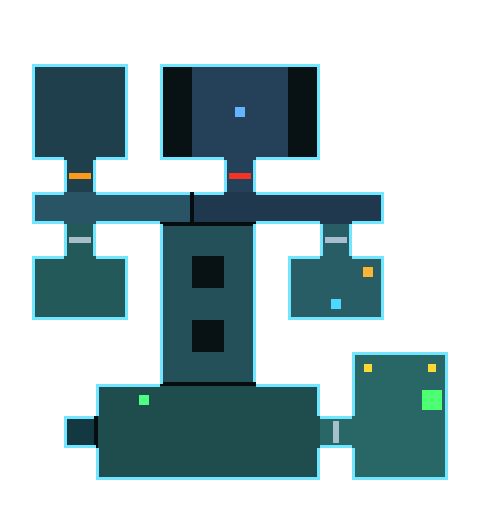
\includegraphics[width=\linewidth]{mapa_01_Mantenimiento.png}
  \end{minipage}
\end{figure}

\FiguraDoble{031_puerta-sin-energia-aviso.jpg}{032_panel-fusibles-reparado.jpg}{fig:panel}{Aviso de la puerta sin energía (izquierda) y panel de fusibles reparado (derecha)}{}

\Figura[0.75\linewidth]{034_puerta-roja-acceso-concedido.jpg}{fig:puertaroja}{La tarjeta roja abre la sala de servidores}{}

\FiguraDoble{063_mantenimiento-decorado.jpg}{064_oficina-seguridad-decorada.jpg}{fig:salas1}{Sala de mantenimiento (izquierda) y oficina de seguridad (derecha) decoradas}{}

\subsubsection{Nivel 2: Pasillos de Almacenamiento}

El segundo nivel fue diseñado y construido por Deisy Lorena Jiménez Martínez con la misma
herramienta de mapas de texto, a partir de un constructor propio del nivel
(Figura~\ref{fig:companera}). Es un laberinto de 21 × 18 celdas (63 × 54~m) formado por tres
franjas de racks en serpentina que se conectan por lados alternos, de modo que hay que recorrerlas
enteras, con salas arriba y abajo (Figura~\ref{fig:mapa2}). La iluminación de los pasillos es de
emergencia, verde y ámbar, con luces que titilan. El nivel empieza con 8:00 de refrigeración y el
núcleo al 86\,\%.

\Figura[0.9\linewidth]{companera_constructor_nivel2.jpg}{fig:companera}{Constructor del Nivel 2 en el editor de Unity}{Captura tomada por D. L. Jiménez Martínez durante la construcción del nivel.}

\begin{enumerate}
  \item La terminal de la sala de inicio da la misión.
  \item La tarjeta roja está en el almacén de carga, al este; abre la oficina de control, donde está
        la tarjeta azul.
  \item La tarjeta azul abre el núcleo de datos, que guarda el Disco Maestro~2.
  \item Con el disco suena la alarma y hay que volver por el laberinto hasta el ascensor, junto al
        inicio.
\end{enumerate}

La sala de respaldo es opcional y tiene la terminal de guardado, una memoria USB y objetos de
curación; la cafetería tiene las máquinas expendedoras. En este nivel aparecen los cuerpos de la
unidad táctica, que dan la pistola, la escopeta y la munición (Figura~\ref{fig:nivel2}). Hay siete
androides entre patrullas y estaciones de carga, con 84 puntos de vida en total, y la munición del
nivel suma unos 97 puntos de daño (26 balas y 5 cartuchos): alcanza para neutralizarlos a todos si
no se desperdicia, pero cada disparo fallado se nota, y lo que sobre pasa al Nivel 3.

\begin{figure}[!htbp]
  \caption{Plano del Nivel 2 generado para el inventario}\label{fig:mapa2}
  \centering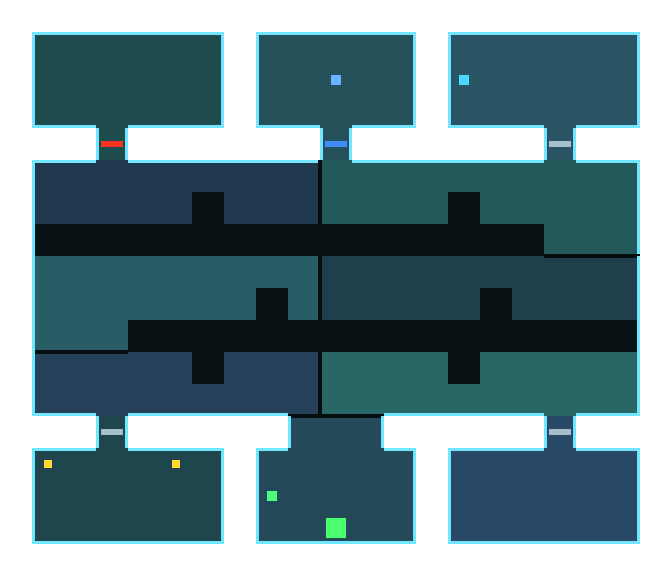
\includegraphics[width=0.6\linewidth]{mapa_02_Almacenamiento.png}
\end{figure}

\FiguraDoble{086_nivel2-sargento-escopeta.jpg}{098_nivel2-estacion-de-carga.jpg}{fig:nivel2}{Nivel 2: el sargento Ortiz con su escopeta (izquierda) y una estación de carga (derecha)}{}

\subsubsection{Nivel 3: Núcleo de Datos}

El último nivel es una sala central enorme y simétrica, con el núcleo en el centro rodeado por un
anillo de racks, tres alas (norte, oeste y este) y la sala de llegada al sur
(Figura~\ref{fig:mapa3}). El temporizador empieza en estado crítico, con 3:00 y el núcleo al
93\,\%. Cuatro androides patrullan en anillos alrededor del núcleo.

\begin{figure}[!htbp]
  \caption{Plano del Nivel 3 generado para el inventario}\label{fig:mapa3}
  \centering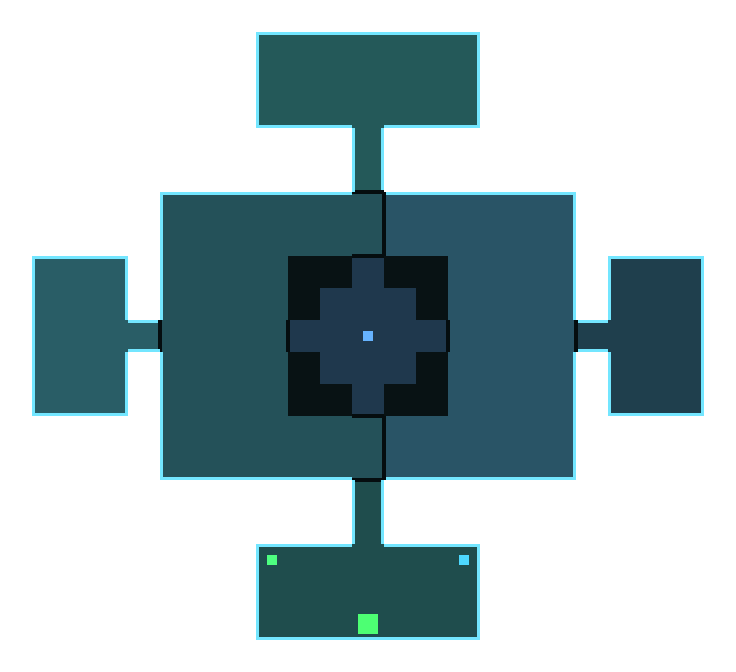
\includegraphics[width=0.6\linewidth]{mapa_03_Nucleo.png}
\end{figure}

El Disco Maestro~3 está protegido por un escudo térmico de tres anillos de energía, que se apaga
con un puzzle: abrir las tres válvulas de refrigeración, una en cada ala, en orden de menor a mayor
presión, como indica el manual de procedimiento de la sala de llegada (Figura~\ref{fig:valvula}).

\begin{itemize}
  \item Cada válvula tiene un manómetro que se lee al acercarse, y las presiones cambian en cada
        partida, por lo que hay que recorrer las alas y comparar.
  \item Si se abre una válvula en orden, la rueda gira, se apaga un tercio del escudo y el núcleo
        gana 60~s, una sola vez por válvula.
  \item Si se abre fuera de orden, se produce una sobrepresión: sale un chorro de vapor, todas las
        válvulas se cierran, el núcleo pierde 15~s y el estruendo atrae a los androides.
  \item Las notas de los cuerpos del nivel dan pistas sobre el orden.
\end{itemize}

\FiguraDoble{099_nivel3-valvula-manometro.jpg}{100_nivel3-alarma-disco.jpg}{fig:valvula}{Válvula del ala este con su manómetro (izquierda) y extracción del Disco Maestro~3 (derecha)}{}

Al tomar el disco se activa el jefe final, descrito en la fase~4. Con el jefe destruido, la salida
de emergencia permite iniciar el reinicio manual, que da paso a la cinemática final y a la pantalla
de Victoria.

\subsubsection{Cinemáticas}

El sistema de cinemáticas (\cod{Cinematica}) se hizo con el propio motor del juego: toma la cámara
y el personaje, muestra barras negras y subtítulos, oculta el HUD y detiene el temporizador y a los
androides. Cada plano define dónde empieza y termina la cámara, que se mueve con suavidad, qué
subtítulo aparece y qué ocurre en escena (caminar, mirar alrededor, abrir o cerrar una puerta,
encender la alarma, despertar a un androide). Los subtítulos usan el nombre del técnico elegido, y
cualquier cinemática se puede saltar. El constructor de niveles arma las cinemáticas a partir del
mapa.

\begin{itemize}
  \item \textbf{Entrada:} el técnico entra por la puerta de servicio, se pregunta \textquote{¿Qué
        pasó aquí\ldots?} mientras mira a su alrededor (con cinemática inversa de cabeza y torso) y
        la puerta se sella detrás de él (Figura~\ref{fig:intro}).
  \item \textbf{Alarma:} al extraer un disco, las luces pasan a rojo y laten, y la cámara muestra a
        las unidades encendiéndose una por una (Figura~\ref{fig:alarma}).
  \item \textbf{Final:} el sistema detecta los tres discos, las luces de alarma se apagan, las
        unidades caen desconectadas y se publican los registros del día 14
        (Figura~\ref{fig:final}).
\end{itemize}

\FiguraDoble{092_intro-puerta-servicio.jpg}{093_intro-que-paso-aqui.jpg}{fig:intro}{Cinemática de entrada: el técnico cruza la puerta de servicio (izquierda) y se pregunta qué pasó (derecha)}{}

\FiguraDoble{095_intro-puerta-sellada.jpg}{096_alarma-luces-rojas.jpg}{fig:alarma}{La puerta de servicio queda sellada (izquierda) y la alarma tiñe de rojo el nivel (derecha)}{}

\FiguraDoble{106_final-reinicio-manual.jpg}{107_final-se-acabo.jpg}{fig:final}{Cinemática final: el reinicio manual (izquierda) y el cierre de la historia (derecha)}{}

\subsubsection{Transición entre niveles}

El paso de un nivel al siguiente es una secuencia animada en el ascensor (Figura~\ref{fig:ascensor}).
Primero, las puertas se recogen hacia los marcos, sale la luz de la cabina y el técnico camina
hacia ella. Luego, el viaje transcurre dentro de una cabina de montacargas construida con primitivas
y con los materiales del propio ascensor, con una cámara fija en una esquina del techo: la cabina
arranca con un tirón, el indicador del panel baja de piso, la luz falla en dos momentos y la luz de
cada piso barre la cabina de abajo hacia arriba, hasta que frena de golpe. Mientras tanto, el nivel
siguiente se carga detrás de una pantalla negra y aparece con el sonido de las puertas y un
fundido. El viaje se puede saltar.

\Figura[0.95\linewidth]{114_transicion-ascensor.jpg}{fig:ascensor}{Las cuatro partes de la transición en el ascensor}{}

\subsubsection{Menú principal}

La escena \cod{00\_Menu} contiene el primer Canvas del juego, sobre un pasillo 3D del centro de
datos con racks y LEDs, los dos técnicos sobre plataformas con anillos de luz y un androide al fondo.
La cámara se mueve sola entre el plano del título y el del selector, como una cámara de seguridad.
El menú tiene cuatro pantallas:

\begin{enumerate}
  \item \textbf{Título} (Figura~\ref{fig:titulo}): logotipo con efecto de falla de pantalla,
        opciones del menú, el logo de la Universidad Central y un aviso de alerta que parpadea. La
        opción \textit{Continuar} aparece cuando hay una partida guardada, y \textit{Salir} se oculta
        en la versión web.
  \item \textbf{Selector de personaje} (Figura~\ref{fig:selector}, izquierda): el técnico elegido recibe un foco
        de luz, su anillo se enciende en cian y gira despacio, y a la izquierda aparece su ficha con
        su habilidad.
  \item \textbf{Informe de la misión} (Figura~\ref{fig:selector}, derecha): explica el objetivo, las amenazas
        y los controles, junto al retrato del técnico, y \textit{Iniciar misión} carga el Nivel~1.
  \item \textbf{Créditos} (Figura~\ref{fig:creditos}): materia, universidad, docente, semestre,
        integrantes y autores de los recursos. Sus textos y logos están en un archivo de datos que
        se edita desde Unity sin tocar el código.
\end{enumerate}

\Figura[0.85\linewidth]{118_titulo-logo-universidad.jpg}{fig:titulo}{Pantalla de título}{}

\FiguraDoble{051_selector-neyder.jpg}{053_briefing-mision.jpg}{fig:selector}{Selector de personaje (izquierda) e informe de la misión (derecha)}{}

\Figura[0.85\linewidth]{119_creditos-completos.jpg}{fig:creditos}{Pantalla de créditos}{}

El personaje elegido pasa al nivel mediante \cod{EstadoPartida}: un componente del jugador coloca
el avatar correspondiente antes que el resto de scripts, y como los dos avatares son Humanoid y
comparten el controlador de animación, el movimiento, las animaciones y la inteligencia artificial
funcionan igual con cualquiera.

\subsubsection{Pantallas de Game Over y Victoria}

El tercer Canvas es la pantalla final, presentada como una falla crítica del sistema Nexus y
animada paso a paso: destello y estática, tres anillos de radar que giran alrededor de un núcleo
que late, un título que se escribe con aberración cromática, el retrato del técnico con la leyenda
\textquote{Señal biométrica perdida}, un registro de terminal que cambia según la causa, un monitor
de pulso que se apaga, un informe del incidente y los comandos para reintentar, cargar la partida o
volver al menú (Figura~\ref{fig:gameover}). La Victoria usa la misma pantalla en verde y cian, con el
pulso estable (Figura~\ref{fig:victoria}). Todos sus gráficos se generan por código.

\FiguraDoble{047_game-over-anomalia-purgada.jpg}{048_game-over-colapso-termico.jpg}{fig:gameover}{Game Over por un androide (izquierda) y por colapso térmico (derecha)}{}

\Figura[0.8\linewidth]{049_victoria-sistema-restaurado.jpg}{fig:victoria}{Pantalla de Victoria}{}

% =====================================================================
\subsection{Fase 7: exportación}

Las tres versiones se compilaron desde el mismo proyecto con los perfiles de la fase~0. Windows usa
el entorno Mono; Android y Web usan IL2CPP, que convierte el código C\# a C++ antes de compilarlo
para procesadores ARM64 o para WebAssembly. Cada versión se probó al terminar: el ejecutable de
Windows se abrió y su registro no mostró errores (Figura~\ref{fig:windows}), y la versión web se
abrió en el navegador a través de un servidor local, porque un juego WebGL no se puede abrir con
doble clic, y se recorrió desde el menú hasta el Nivel~1 sin errores en la consola
(Figura~\ref{fig:web}). La plantilla web incluye el botón de pantalla completa que se necesita para
incrustar el juego en el artículo. La Tabla~\ref{tab:builds} resume las versiones finales.

\begin{TablaAPA}{tab:builds}{Versiones finales del juego}
\begin{tabularx}{\linewidth}{P{2.6cm}LP{2cm}P{2.4cm}}
\toprule
Plataforma & Archivo de entrega & Tamaño & Compilación \\
\midrule
Windows & \cod{Nexus\_Windows.zip} con \cod{Nexus.exe} & 97 MB & 0 errores \\
Android & \cod{Nexus.apk} (Android 8.0 o posterior, ARM64) & 75 MB & 0 errores \\
Web (WebGL) & \cod{Nexus\_Web.zip} para publicar en un servidor & 68 MB & 0 errores \\
\bottomrule
\end{tabularx}
\end{TablaAPA}

\Figura[0.8\linewidth]{windows_exe_menu.jpg}{fig:windows}{El juego ejecutándose en Windows}{}

\FiguraDoble{116_build-webgl-final-menu.jpg}{117_build-webgl-final-nivel1.jpg}{fig:web}{La versión web en el navegador: menú con el botón de pantalla completa (izquierda) y Nivel~1 (derecha)}{}

\section{Resultados}

El juego final cumple todos los requisitos de la asignatura (Tabla~\ref{tab:requisitos}) y se
entrega en las tres plataformas pedidas.

\begin{TablaAPA}{tab:requisitos}{Cumplimiento de los requisitos de la asignatura}
\begin{tabularx}{\linewidth}{P{4.6cm}L}
\toprule
Requisito & Cómo lo cumple Nexus \\
\midrule
Tres niveles jugables con progresión lógica & Cuarto de Mantenimiento, Pasillos de Almacenamiento y Núcleo de Datos; cada uno se desbloquea al extraer el disco del anterior \\
Tres Canvas diferenciados & Menú principal, HUD y pantalla de Game Over y Victoria, además del inventario \\
Selector de personajes con Avatar Humanoid & Avatares de los dos integrantes configurados como Humanoid, con un único controlador de animación \\
Música de fondo con componentes de audio & Música por capas (menú, exploración, tensión, jefe, alarma y victoria) y ambiente del centro de datos \\
Créditos e imagen institucional & Pantalla de créditos con la materia, la Universidad Central, el docente y los integrantes; logo en el título y en los créditos \\
Explicación del objetivo & Informe de la misión antes del Nivel~1 y objetivo actual en el HUD \\
Temporizador & Refrigeración con cuenta atrás y temperatura del núcleo \\
Sistema de vidas o salud & Tres oportunidades de evasión con estado herido y objetos de curación \\
Objetos coleccionables con contador & Discos Duros Maestros (x/3) y cartuchos de refrigerante \\
Inteligencia artificial autónoma & Androides con patrulla, visión, oído, persecución y búsqueda sobre una malla de navegación, y un jefe final \\
Cuadros de diálogo narrativos & Terminales, notas, avisos del sistema y subtítulos de las cinemáticas \\
Plataformas & Windows (\cod{.exe}), WebGL con pantalla completa y Android (\cod{.apk}) \\
\bottomrule
\end{tabularx}
\end{TablaAPA}

Además de los requisitos, el juego incorpora una habilidad distinta para cada personaje, armas con
munición limitada y apuntado asistido, cadáveres que se registran con notas que cuentan la historia,
animaciones de escopeta creadas por código, cámaras que guían al jugador hacia los objetos
importantes, un inventario con archivo y mapa, guardado en terminales, máquinas expendedoras con
riesgo, un puzzle de válvulas, un jefe final, cinemáticas hechas con el motor, una transición
animada entre niveles y controles táctiles.

\section{Conclusiones}

El desarrollo por fases, con una versión jugable al final de cada una y compilaciones de prueba
desde el inicio, permitió construir un juego completo de tres niveles y llevarlo a las tres
plataformas sin sorpresas al final del proyecto.

La construcción del contenido mediante herramientas de editor programadas fue la decisión que más
influyó en el resultado. Describir los niveles como mapas de texto y generar texturas, objetos,
decoración, cámaras y cinemáticas por código hizo posible producir escenarios grandes y coherentes
con un equipo de dos personas, y aplicar cualquier ajuste de diseño en todo el juego con solo
reconstruir.

El sistema de Avatar Humanoid de Unity fue la base del trabajo de personajes: permitió que los
avatares de los integrantes, los androides y los personajes secundarios compartieran animaciones,
y que el selector de personajes funcionara con un único controlador. Ese mismo sistema hizo posible
crear poses y animaciones nuevas músculo por músculo, como las de los cadáveres y la escopeta.

Las referencias del survival horror clásico orientaron las decisiones de diseño: cámaras fijas que
cortan cuando el personaje sale del cuadro, controles tipo tanque, recursos escasos, sigilo frente
a enemigos que ven y oyen, y una mezcla de audio que acompaña la tensión de cada situación.

Finalmente, adaptar el juego a celulares y navegadores exigió cuidar el rendimiento desde el
principio (mallas combinadas, sombreadores sin scripts, una sola cámara activa) y añadir controles
táctiles, lo que dejó un juego que se puede jugar de la misma forma en las tres plataformas.


\clearpage
\printbibliography[heading=bibintoc,title=Referencias]

% Anexos (después de las referencias, cada uno en una página nueva)
\newcommand{\Anexo}[2]{%
  \clearpage
  \phantomsection\addcontentsline{toc}{section}{Anexo #1. #2}
  \begin{center}\textbf{Anexo #1}\\[0.5\baselineskip]\textbf{#2}\end{center}}

\Anexo{A}{Controles del juego}

El juego se controla con teclado y ratón, con un mando compatible con Windows o con la pantalla
táctil en Android y en el navegador del celular (Tabla~\ref{tab:controles-completos}).

\begin{TablaAPA}{tab:controles-completos}{Controles del juego en las tres formas de entrada}
\begin{tabularx}{\linewidth}{P{3.6cm}P{3.6cm}P{3.2cm}L}
\toprule
Acción & Teclado y ratón & Mando & Pantalla táctil \\
\midrule
Avanzar / retroceder & \tecla{W} / \tecla{S} & Stick izquierdo & Joystick arriba / abajo \\
Girar & \tecla{A} / \tecla{D} & Stick izquierdo & Joystick a los lados \\
Correr & \tecla{Shift} & Presionar el stick & CORRER \\
Media vuelta & \tecla{Shift + S} & --- & CORRER y joystick abajo \\
Interactuar & \tecla{E} & Botón Y & INTERACTUAR \\
Habilidad & \tecla{Q} & Botón X & HABILIDAD \\
Inventario & \tecla{Tab} o \tecla{I} & Start & INVENTARIO \\
Cambiar de arma & \tecla{1}, \tecla{2}, \tecla{3}; \tecla{0} guarda & Cruceta & ARMA \\
Apuntar & Clic derecho o \tecla{K} & Gatillo izquierdo & APUNTAR \\
Disparar o atacar & Clic izquierdo o \tecla{J} & Gatillo derecho & DISPARAR o ATACAR \\
Recargar & \tecla{R} & Botón superior derecho & RECARGAR \\
Avanzar diálogos & \tecla{E}, \tecla{Espacio}, \tecla{Enter} o clic & Botón A o Y & Tocar la pantalla \\
Saltar cinemática & \tecla{Enter}, \tecla{Esc} o \tecla{Espacio} & Start & Tocar la pantalla \\
\bottomrule
\end{tabularx}
\end{TablaAPA}

\Anexo{B}{Créditos de los recursos de terceros}

Los modelos de las armas se tomaron de Sketchfab con licencia CC BY 4.0, que exige citar a sus
autores \parencite{ccby40}; la música y los efectos, de Pixabay \parencite{pixabaylicencia}. Todo lo
demás (escenarios, objetos, texturas, sombreadores, interfaz y efectos visuales) se creó para este
proyecto.

\begin{TablaAPA}{tab:creditos-modelos}{Modelos 3D y personajes de terceros}
\begin{tabularx}{\linewidth}{P{4.4cm}LP{3.4cm}}
\toprule
Uso en el juego & Recurso & Autor o fuente \\
\midrule
Bayoneta & \textit{M9 Bayonet} \parencite{erdogay_m9} & Atilla Kutluay Erdoğay \\
Pistola & \textit{Beretta M9A1} \parencite{do_m9a1} & Hung Do \\
Escopeta & \textit{Remington 870 Shotgun} \parencite{milin_870} & Andrei Milin \\
Avatares de los integrantes & Avatares generados desde fotografías & Avaturn \\
Androides, operadores, empleado y animaciones & Y Bot, personajes y animaciones & Mixamo (Adobe) \\
\bottomrule
\end{tabularx}
\end{TablaAPA}

\begin{TablaAPA}{tab:creditos-efectos}{Efectos de sonido (Pixabay)}
\begin{tabularx}{\linewidth}{P{5.2cm}LP{4.3cm}}
\toprule
Uso en el juego & Sonido & Autor \\
\midrule
Disparo de pistola & 9mm Pistol Shot & freesound\_community \\
Disparo de escopeta & Shotgun Firing 3 & freesound\_community \\
Bombeo de la escopeta & Pump Action Shotgun Cycle & freesound\_community \\
Recarga de pistola & 1911 Reload & freesound\_community \\
Cartucho de escopeta & Shell Load & freesound\_community \\
Sin munición & Dry Fire & spinopel \\
Bayoneta & Sword Slash 01 & u\_xjrmmgxfru \\
Bala contra el blindaje & Bullet Hit Metal & freesound\_community \\
Un androide detecta al técnico & Distorted Stinger & ALEXIS\_GAMING\_CAM \\
Pisada del androide & Big Robot Footstep 015 & AudioPapkin \\
Un androide se enciende & Wake Up the Robot & freesound\_community \\
Un androide cae o se apaga & Robot Power Off & freesound\_community \\
Pisadas del técnico & Concrete Footsteps 1 & freesound\_community \\
Neyder herido & Male Grunting in Pain & freesound\_community \\
Deisy herida & Female Hurt 2 & freesound\_community \\
Puertas de seguridad & Sci-Fi Heavy Hydraulic Door & SoundEffectsParty \\
Recoger un objeto & Item Pickup & freesound\_community \\
Navegar por los menús & Old Computer Click & Finntastico \\
Mensajes de terminal e inventario & Radio Static Break & ZenoWaves \\
Válvula que gira & Long Metal Creak & freesound\_community \\
Vapor de la válvula & Steam Hissing & DRAGON-STUDIO \\
Carga del jefe & Energy Charge 2 & Yodguard \\
Descarga del jefe & Electro Impact & zehendrew \\
Máquina expendedora & Vending Machine & freesound\_community \\
Señuelo de red & FM Radio Static & freesound\_community \\
Sirena de la alarma & Facility Siren (loopable) & freesound\_community \\
Game Over & Dramatic Synth Echo & freesound\_community \\
Ascensor: puertas, marcha y frenada & 080223-002 Freight Elevator & freesound\_community \\
\bottomrule
\end{tabularx}
\end{TablaAPA}


\end{document}
